\documentclass{bmstu}


\usepackage{physics}
\usepackage{pdfpages}
\usepackage{tabularx}
\usepackage{longtable}
\usepackage{xfrac}
\usepackage{amssymb}
\usepackage{dsfont}
\usepackage{upgreek}
\usepackage{color, colortbl}
\usepackage{listings}
\usepackage{ amssymb }
\usepackage{tikz}
\usepackage{mathtools}
\usepackage{amsmath}

\graphicspath{
	{graphics/}
}

\begin{document}
\section*{01/11}
\begin{center}
\underline{Конечные элементы более высокого порядка}

\underline{Одномерные квадратичные и кубические функции}
\end{center}
\[
\varphi = \alpha_1 + \alpha_2x, \ \dim L = 1, n = 2 \text{ -- симплекс элементы.}
\]

Комплекс элементы -- количество узлов n > 2.  

\begin{center}
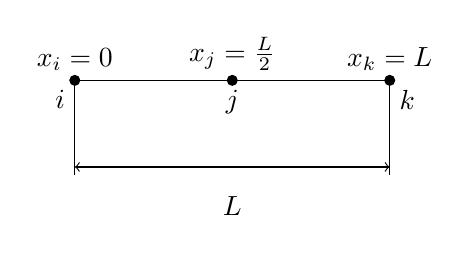
\begin{tikzpicture}[scale=2]
\draw (-1,0) -- (1,0);
\fill (-1,0) circle (1pt) node[below left]{$i$} node[above]{$x_i = 0$};
\fill (0,0) circle (1pt) node[below]{$j$} node[above]{$x_j = \frac{L}{2}$};
\fill (1,0) circle (1pt) node[below right]{$k$} node[above]{$x_k = L$};
\draw (-1,0) -- (-1, -0.6);
\draw (1,0) -- (1, -0.6);
\draw[<->] (-1, -0.55) -- (1, -0.55);
\node at (0, -0.8) {$L$};
\end{tikzpicture}
\end{center}

$\varphi = \alpha_1 + \alpha_2x + \alpha_3x^2 = N \Phi$

В общем виде: $\varphi = \alpha_1 + \alpha_2x + \cdots + \alpha_nx^{n-1}$
\[
\begin{cases}
\Phi_i = \alpha_1 + \alpha_2x_i + \alpha_2x^{2}_i \\
\Phi_j = \alpha_1 + \alpha_2x_j + \alpha_2x^{2}_j \\
\Phi_k = \alpha_1 + \alpha_2x_k + \alpha_2x^{2}_k \\
\end{cases}
\rightarrow \alpha_1, \alpha_2, \alpha_3
\]
\[
\alpha_1 = \Phi_i, \ \alpha_2 = \frac{-3\Phi_i + 4\Phi_j -\Phi_k}{L}, \ \alpha_3 = \frac{2(\Phi_i-2\Phi_j+\Phi_k)}{L^2}
\]
\[
\varphi = \alpha_1 + \alpha_2x + \alpha_3x^2 = 
\]
\[
 = \Phi_i   \underbrace{\left(1 - \frac{3x}{L} + \frac{2x^2}{L^2} \right) }_{N_i}   + \Phi_j \underbrace{\left(\frac{4x}{L} - \frac{4x^2}{L^2} \right)}_{N_j} + \Phi_k \underbrace{\left(-\frac{x}{L} + \frac{2x^2}{L^2} \right)}_{N_k} = 
\]
\[
 = N_i \Phi_i + N_j \Phi_j + N_k \Phi_k = [N]\{\Phi\}
\]
\[
N_i = 1 - \frac{3x}{L} + \frac{2x^2}{L^2}, \ N_j = \frac{4x}{L} - \frac{4x^2}{L^2}, \ N_k = -\frac{x}{L} + \frac{2x^2}{L^2}
\]

Этот же результат можно получить без использования системы уравнений. Зададим в узлах пробные функции $f_{\alpha},\ \alpha \in \{i, j, k\}$, такие, что $f_{\alpha}(x_{\alpha}) = 0$:

\begin{center}
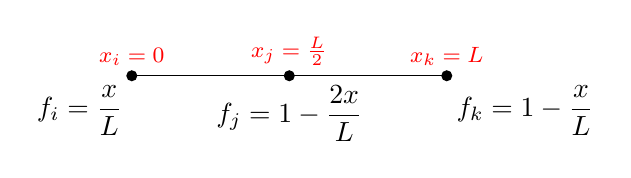
\begin{tikzpicture}[scale=2]
\draw (-1,0) -- (1,0);
\fill (-1,0) circle (1pt) node[below left]{$\displaystyle f_i = \frac{x}{L}$} node[above][red]{\footnotesize$x_i = 0$};
\fill (0,0) circle (1pt) node[below]{$\displaystyle f_j = 1-\frac{2x}{L}$} node[above][red]{\footnotesize$x_j = \frac{L}{2}$};
\fill (1,0) circle (1pt) node[below right]{$\displaystyle f_k = 1-\frac{x}{L}$} node[above][red]{\footnotesize$x_k = L$};
\end{tikzpicture}
\end{center}

Формулы для нахождения функций форм: 
\[
N_i = \frac{f_jf_k}{f_jf_k|_{x = x_i=0}}, \ N_j = \frac{f_if_k}{f_if_k|_{x = x_j=\frac{L}{2}}}, \ N_k = \frac{f_if_j}{f_if_j|_{x = x_k = L}}
\]
\[
N_i = \left(1 - \frac{2x}{L}\right)\cdot \left( 1 - \frac{x}{L} \right), \ N_j = \frac{4x}{L} \cdot \left( 1 - \frac{x}{L}\right), \ N_k = -\frac{x}{L}\cdot \left(1 - \frac{2x}{L}\right)
\]

Аналогично можно найти функции формы для конечных элементов более высокого порядка:
\[\varphi = \alpha_1 + \alpha_2x + \alpha_3x^2 + \alpha_4x^3 = N_i\Phi_i,\ i = 1,\dots, 4\]
\begin{center}
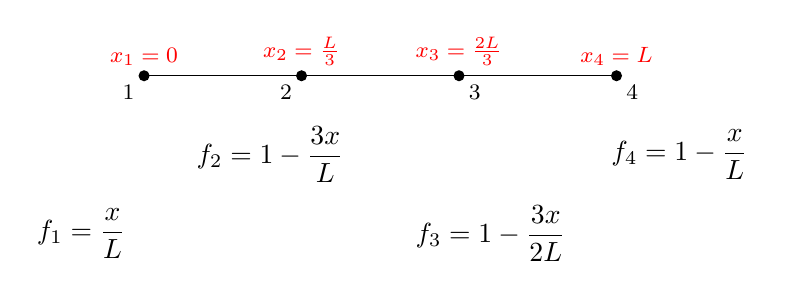
\begin{tikzpicture}[scale=2]
\draw (-1,0) -- (2,0);
\fill (-1,0) circle (1pt) node[below left]{\footnotesize1} node[above][red]{\footnotesize$x_1 = 0$};
\fill (0,0) circle (1pt) node[below left]{\footnotesize2} node[above][red]{\footnotesize$x_2 = \frac{L}{3}$};
\fill (1,0) circle (1pt) node[below right]{\footnotesize3} node[above][red]{\footnotesize$x_3 =  \frac{2L}{3}$};
\fill (2,0) circle (1pt) node[below right]{\footnotesize4} node[above][red]{\footnotesize$x_4 = L$};
\node at (-1.4,-1) {$\displaystyle f_1 = \frac{x}{L}$};
\node at (-0.2,-0.5) {$\displaystyle f_2 = 1 - \frac{3x}{L}$};
\node at (1.2,-1) {$\displaystyle f_3 = 1 - \frac{3x}{2L}$};
\node at (2.4,-0.5) {$\displaystyle f_4 = 1 - \frac{x}{L}$};
\end{tikzpicture}
\end{center}

\begin{center}
\underline{Постановка задачи}
\end{center}
\[K^{(e)} q = P^{(e)}\]
\[K^{(e)} = \int \limits_V B^T D B dV + \int \limits_S \alpha_g N^T N dS\]
\[P^{(e)} = \int \limits_V f N^T dV - \int \limits_S q N^T dS + \int \limits_S \alpha_g T_g N^T dS\]
\[dV = Sdx,\ \ dS = Pdx,\ \text{где } P \text{ -- периметр}\]
\[B = \frac{d[N]}{dx} = \left[ \frac{dN_i}{dx},\ \  \frac{dN_j}{dx},\ \  \frac{dN_k}{dx}\right] = \left[ -\frac{3}{L} + \frac{4x}{L^2},\ \  \frac{4}{L} - \frac{8x}{L^2},\ \  -\frac{1}{L} + \frac{4x}{L^2}\right]\]
\[D = k_x, \text{ так как задача одномерная}\]
Получаем:
\[\int \limits_V B^T D B dV = S k_x \cdot \int \limits_0^L  B^T B dx =\]
\[= Sk_x \cdot \int \limits_0^L
\begin{bmatrix}
\left(-\frac{3}{L} + \frac{4x}{L^2} \right)^2 & \left(-\frac{3}{L} + \frac{4x}{L^2} \right)\left(\frac{4}{L} - \frac{8x}{L^2} \right) & \left(-\frac{3}{L} + \frac{4x}{L^2} \right)\left(-\frac{1}{L} + \frac{4x}{L^2} \right) \\
\left(-\frac{3}{L} + \frac{4x}{L^2} \right)\left(\frac{4}{L} - \frac{8x}{L^2} \right) & \left(\frac{4}{L} - \frac{8x}{L^2} \right)^2 & \left(\frac{4}{L} - \frac{8x}{L^2} \right)\left(-\frac{1}{L} + \frac{4x}{L^2} \right)\\
\left(-\frac{3}{L} + \frac{4x}{L^2} \right)\left(-\frac{1}{L} + \frac{4x}{L^2} \right)& \left(\frac{4}{L} - \frac{8x}{L^2} \right)\left(-\frac{1}{L} + \frac{4x}{L^2} \right) & \left(-\frac{1}{L} + \frac{4x}{L^2} \right)^2
\end{bmatrix} dx =\]
\[= \frac{Sk_x}{6L} \cdot 
\begin{bmatrix}
14 & -16 & 2\\
-16 & 32 & -16\\
2 & -16 & 14
\end{bmatrix}\]

Рассмотрим следующий интеграл:
\[\int \limits_S \alpha_g N^T N dS = P \alpha_g \cdot \int \limits_0^L N^T N dx = P \alpha_g
\cdot \int \limits_0^L \begin{bmatrix}
N_i^2 & N_iN_j & N_iN_k \\
N_iN_j & N_j^2 & N_jN_k \\
N_iN_k & N_jN_k & N_k^2 \\
\end{bmatrix} dx = \]
\[= \frac{\alpha_g З L}{30} \cdot \begin{bmatrix}
4 & 2 & -1 \\
2 & 16 & 2 \\
-1 & 2 & 4 \\
\end{bmatrix}\]

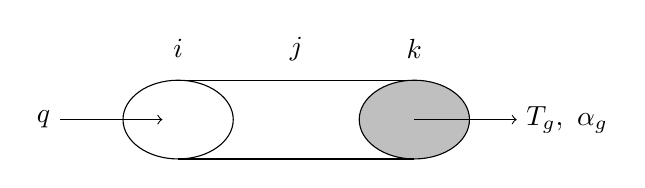
\begin{tikzpicture}
    % Рисуем основу цилиндра
    \fill[gray!50] (2,0) circle (0.7 and 0.5); % закрашенная правая сторона
    \draw (-1,0) ellipse (0.7 and 0.5); % передняя окружность
    \draw (2,0) ellipse (0.7 and 0.5); % задняя окружность

    % Рисуем боковые линии
    \draw (-1,0.5) -- (2,0.5); % нижняя боковая линия
    \draw (-1,-0.5) -- (2,-0.5); % верхняя боковая линия
    
    \node at (-1, 0.9) {$i$};
    \node at (0.5, 0.9) {$j$};
    \node at (2, 0.9) {$k$};
    
    \draw[<-] (-1.2,0) -- (-2.5,0) node[left] {$q$};
    \draw[->] (2,0) -- (3.3,0) node[right] {$T_g,\ \alpha_g$};
\end{tikzpicture}






























\end{document}